\documentclass[11pt, oneside]{article}   	% use "amsart" instead of "article" for AMSLaTeX format
\usepackage{geometry}                		% See geometry.pdf to learn the layout options. There are lots.
\geometry{letterpaper}                   		% ... or a4paper or a5paper or ... 
%\geometry{landscape}                		% Activate for rotated page geometry
%\usepackage[parfill]{parskip}    		% Activate to begin paragraphs with an empty line rather than an indent
\usepackage{graphicx}				% Use pdf, png, jpg, or eps§ with pdflatex; use eps in DVI mode
								% TeX will automatically convert eps --> pdf in pdflatex		
\usepackage{amssymb,amsmath}
\usepackage{stmaryrd}
\usepackage{subcaption}
\graphicspath{ {\string~/Desktop/AM900/a3/latex} }

%SetFonts

%SetFonts


\title{AM900: Space-time Discontinuous Galerkin for the Advection Equation}
\author{Martin Pham}
\date{Fall 2017}							% Activate to display a given date or no date

\begin{document}
\maketitle

\begin{center}
Acknowledgements: Keegan Kirk and Abdullah Sivas for time and guidance debugging
\end{center}

%%%%%%%%%%%%%%%%%%%%%%%%%
\section{Formulation}
%
% COMPUTATIONAL DOMAIN
%
\subsection{Computational Domain}
For a space-time variable $x = (t,\bar{x})$ and some constant $a$, consider the advection problem
\begin{equation} \label{og_prob}
\begin{split}
\partial_t u + a \partial_x u &= f \qquad\qquad \mathcal{E} \subset \mathbb{R}^{1+1}\\
u(\bar{x}, t_0) &= u_{0}(\bar{x}) \qquad \Omega(t) \in \mathbb{R}
\end{split}
\end{equation}
The space-time domain is $\mathcal{E} \subset \mathbb{R}^2$ and the spatial flow domain $\Omega$ at some time $t$ is
\[\Omega(t) = \{ \bar{x} \in \mathbb{R} : (t,\bar{x}) \in \mathcal{E}\}\]
The initial flow domain is $\Omega(t_0)$ and the final domain $\Omega(T)$ for some final time $T$.
Partition the time part of the domain $[t_0,T]$ into $N$ intervals $I_n = (t_n, t_{n+1})$ with $\Delta t_n = t_{n+1} - t_n$ and  $t_0 < t_1 < ... < t_N = T$.
Define the space-time slab at $t_n$ as $\mathcal{E}^n = \mathcal{E} \cap I_n$.
We may then partition the space-time domain into slabs, $\mathcal{E} = \bigcup_{n=1}^{N} \mathcal{E}^n$.\\
For a space-time slab $\mathcal{E}^n$, the bottom and top of the slab are specified by $\Omega(t_n)$ and $\Omega(t_{n+1})$ respectively.
The sides of the time slab are on the boundary of $\mathcal{E}$ and are specified by 
\[\mathcal{Q}^n = \partial \mathcal{E} \setminus (\Omega(t_n) \cup \Omega(t_{n+1}))\]
Let $\mathcal{T}^n = \{K_j^n\}$ be the tessellation of a flow domain $\Omega(t_n) = \bigcup_{j=1}^{M} K_j^n$.
We then tesselate a slab $\mathcal{E}^n$ by linear interpolation in time between the spatial tessellations $\mathcal{T}^n$ and $\mathcal{T}^{n+1}$.
A space-time element $\mathcal{K}_j^n$ is obtained by connecting the spatial elements $K_j^n \subset \Omega(t_n)$ and $K_j^{n+1} \subset \Omega(t_{n+1})$.
At time $t_n$  a slab may be considered $\mathcal{E}^n = \bigcup_{j=1}^{M} \mathcal{K}_j^n$ with tessellation $\mathcal{T}^n = \{\mathcal{K}_j^n\}$.
The entire computational domain is then  $\mathcal{T} = \bigcup_{n=1}^{N} \mathcal{T}^n$.


%
% REFERENCE ELEMENT
%
\subsection{Reference Elements}
In order to compute the integral terms in the weak form of the problem, we desire to map elements to some master reference element which may define our quadrature rules for integration.
Note that quadrature rules should be of sufficient order as other approximations in the scheme.\\
Let the space-time reference variable be $\xi = (\xi_0,\bar{\xi})$ with space-time reference element $\hat{\mathcal{K}} = (-1,1)^2$ and spatial reference element $\hat{K} = (-1,1)$.
At time $t_n$, for some spatial elements $K_j^n$ and $K_j^{n+1}$ we define respectively the mappings
\begin{gather*}
F_K^n : \hat{\mathcal{K}} \rightarrow K_j^n : \bar{\xi} \rightarrow \bar{x} = \sum_{i=1}^2 x_i(K_j^n) \chi_i((\bar{\xi}))\\
F_K^{n+1} : \hat{\mathcal{K}} \rightarrow K_j^{n+1} : \bar{\xi} \rightarrow \bar{x} = \sum_{i=1}^2 x_i(K_j^{n+1}) \chi_i((\bar{\xi}))
\end{gather*}
where the shape functions $\chi_i$ are given by
\[ \chi_1(\bar{\xi}) = \frac{1}{2}(1-\bar{\xi}) \qquad\qquad \chi_2(\bar{\xi}) = \frac{1}{2}(1+\bar{\xi}) \]
and the points $x_i(K_j^n)$ and $x_i(K_j^{n+1})$ are given by the movement of the mesh at time $t_n$ and $t_{n+1}$ respectively.\\
For a space-time element $\mathcal{K}_j^n$ we define the mapping
\begin{equation*}
G_{\mathcal{K}_j}^n : \hat{\mathcal{K}} \rightarrow \mathcal{K}_j^n : \xi \rightarrow x =
\bigg( \frac{1}{2} (t_{n+1} + t_n) + \frac{1}{2} (t_{n+1} - t_n) \xi_0 \quad,\quad
\frac{1}{2} (1-\xi_0) F_K^n(\bar{\xi}) + \frac{1}{2} (1+\xi_0) F_K^{n+1}(\bar{\xi}) \bigg)
\end{equation*}


%
% WEAK FORM
%
\subsection{Weak Form}
Define the space-time gradient operator and flux
\[ \nabla = (\partial_t, \partial_x) \qquad\qquad \mathcal{F}(u) = (u, au) \]
Then the differential equation in \eqref{og_prob} becomes
\begin{equation}\label{st_og_prob}
 \nabla \cdot \mathcal{F} = f 
\end{equation}
To obtain the weak form, we multiply \eqref{st_og_prob} by a sufficiently smooth test function $v$ and integrate by parts over a single element.
Since the basis functions of the finite dimensional approximation spaces will be discontinuous, we may consider the equations over a sum of elements of the computational domain.
The problem becomes
\begin{equation}\label{st_prob}
 \sum_{\mathcal{K} \in \mathcal{T}} \bigg[ \int_{\mathcal{K}}\nabla v \cdot\mathcal{F}dx + \int_{\partial\mathcal{K}}v\mathcal{F}\cdot nds \bigg]  = 
 \int_{\mathcal{K}} v f dx
\end{equation}
The second integral term is replaced by an approximation of the flux $\mathcal{F}$ using a numerical flux $\hat{\mathcal{F}}$ that will consider both sides of the solution across discontinuities between elements.
On a space-time element, define the grid-dependent space-time normal that is consistent with a causality in time argument as
\[ n = \begin{cases}
	(-1,0) & K_j^n(t_{n}^+)\\
	(1,0) & K_j^{n+1}(t_{n+1}^-)\\
	(-v_g \bar{n}, \bar{n}) & \mathcal{Q}_j^n\\
	\end{cases} \]
where the grid velocity is $v_g = \frac{\Delta x}{\Delta t} = \frac{x_j^{n+1} - x_j^n}{\Delta t}$.
The second integral term in \eqref{st_prob} may thus be split into separate integrals over different space-time element faces
\begin{equation}\label{split_facets}
\int_{\partial\mathcal{K}} v \mathcal{F}\cdot n ds =
\int_{K_j^n} v \hat{\mathcal{F}} \cdot n d\bar{x} + \int_{K_j^{n+1}} v \hat{\mathcal{F}} \cdot n d\bar{x} + \int_{\mathcal{Q}_j^n} v \hat{\mathcal{F}} \cdot n ds
\end{equation}
Since the solution is double-valued at points of discontinuity across elements, we introduce the approximation of $u$ at these points as
\[ \hat{u} = \begin{cases}
	u_R & K_j^n\\
	u_L & K_j^{n+1}\\
	\end{cases} \]
where the R and L subscripts are to denote respectively the outside and inside of a current element.
This choice is made to be consistent with causality in time at the tops and bottom of a space-time slab.
The integrals in \eqref{split_facets} may then be written as
\begin{equation}\label{double_value}
\begin{split}
\int_{\partial\mathcal{K}} v \mathcal{F}\cdot n ds
&= - \int_{K_j^n} v \hat{u} d\bar{x} + \int_{K_j^{n+1}} v \hat{u} d\bar{x} + \int_{\mathcal{Q}_j^n} v \widehat{(a u - v_g u)} \bar{n} ds\\
&= - \int_{K_j^n} v u_R d\bar{x} + \int_{K_j^{n+1}} v u_L d\bar{x} + \int_{\mathcal{Q}_j^n} v \widehat{(a u - v_g u)} \bar{n} ds\\
\end{split}
\end{equation}
Denote the jump and average operators as
\[ \llbracket \cdot \rrbracket = (\cdot)_L\bar{n_L} + (\cdot)_R\bar{n_R} = ((\cdot)_L - (\cdot)_R)\bar{n_L} \]
\[ \{ \cdot \} = \frac{1}{2}(\cdot_L + \cdot_R) \]
and denote the approximation $\widehat{(au-v_{g}u)}\bar{n}$ as $\hat{g}(u_L,u_R)$.
Since the solution on shared element facets $S$ are double-valued, the last integral term in \eqref{double_value} summed over facets of the slab at $t_n$ may be written as
\begin{equation}\label{facet_integrals}
\begin{split}
\sum_{j=1}^{M} \int_{\mathcal{Q}_j^n} v \widehat{(a u - v_g u)} \bar{n} ds
&= \sum_{j=1}^{M} \int_{\mathcal{Q}_j^n} v \hat{g}(u_L,u_R) ds \\
&= \sum_{S \in S^n} \int_{S} \llbracket v \hat{g}(u_L,u_R) \rrbracket ds \\
&= \sum_{S \in S^n} \int_{S} \llbracket v \rrbracket \hat{g}(u_L,u_R) ds \\
&= \sum_{S \in S^n} \int_{S} (v_L - v_R) \bar{n}_L \hat{g}(u_L,u_R) ds \\
&= \sum_{S \in S^n} \int_{S} (v_L - v_R) \hat{f}(u_L,u_R) ds \\
\end{split}
\end{equation}
where $\hat{f}(u_L,u_R) = \hat{g}(u_L,u_R)\bar{n}_L$.
We choose the upwind flux
\[ \hat{f}(u_L,u_R) = (a-v_g)\bar{n}\{ u \} + \frac{1}{2}|(a-v_g)\bar{n}| \llbracket u \rrbracket \]
Note that if there is no grid motion, $\bar{n}$ becomes a unit normal
\[|(-v_g \bar{n}, \bar{n})| = 1 \iff v_g^2\bar{n}^2 = 1 \iff |\bar{n}| = \frac{1}{\sqrt{1+v_g^2}} = \frac{1}{\sqrt{1+(\frac{\Delta x}{\Delta t})^2}} \]
Note that the left-most facet and right-most facet require special treatment dependant on the direction of the advection, no jump in test functions is imposed.\\
Consider the problem \eqref{st_prob}, applying our integral terms from \eqref{double_value} and \eqref{facet_integrals} we obtain
\begin{small}
\[\sum_{\mathcal{K}\in\mathcal{T}} 
\bigg[ - \int_{\mathcal{K}} \nabla v \cdot \mathcal{F} dx + \int_{K_j^{n+1}} v_L u_L d\bar{x} - \int_{K_j^n} v_L u_R d\bar{x} \bigg]
+ \sum_{\forall S} \int_S (v_L - v_R) \hat{f}(u_L,u_R)ds  =  \int_{\mathcal{K}} v f dx  \]
\end{small}
Splitting the computational domain into space-time slabs
\begin{small}
\[\sum_{n=0}^{N-1} 
\bigg[ \sum_{\mathcal{K}\in\mathcal{T}^n}  
	\bigg(- \int_{\mathcal{K}} \nabla v \cdot \mathcal{F} dx + \int_{K_j^{n+1}} v_L u_L d\bar{x} - \int_{K_j^n} v_L u_R d\bar{x}  \bigg)
	+ \sum_{S \in S^n} \int_S (v_L - v_R) \hat{f}(u_L,u_R)ds \bigg] =  \int_{\mathcal{K}} v f dx \]
\end{small}
We may use the solution obtained from a previous slab (evaluated at the bottom of the current slab) as the initial conditions for the current slab.
Thus we may consider each slab sequentially. The problem becomes: finding $u$ such that for all test functions $v$, the following holds for all $n$
\begin{equation}\label{st_weakform}
\sum_{\mathcal{K}\in\mathcal{T}^n}  
	\bigg(- \int_{\mathcal{K}} \nabla v \cdot \mathcal{F} dx + \int_{K_j^{n+1}} v_L u_L d\bar{x} - \int_{K_j^n} v_L u_R d\bar{x}  \bigg)
	+ \sum_{S \in S^n} \int_S (v_L - v_R) \hat{f}(u_L,u_R)ds = \int_{\mathcal{K}} v f dx 
\end{equation}

\clearpage
%
%POLYNOMIAL EXPANSION
%
\subsection{Polynomial Expansion Coefficients}
We introduce a finite dimensional polynomial basis in order to obtain an approximation to our solution.
The functions $u$ and $v$ may then be expressed in a polynomial basis expansion, the expansion coefficients being the degrees of freedom which we solve for.
The degrees of freedom for a solution in the element $\mathcal{K}_j$ are local (the neighbouring elements and itself) due to the choice of basis functions existing only on a single element.
Approximate $u,v$ from the space
\[ u,v \in V^k = \{u \in L^2(\mathcal{K}_j) : u|_{\mathcal{K}_j} \in P^k(\mathcal{K}_j) \} \]
for $k$ the highest degree Legendre polynomial basis function on element $\mathcal{K}_j$.
We choose a linear polynomial approximation $k=1$.
On the reference element $\hat{\mathcal{K}_j} = (-1,1)^2$, we define the basis functions $\Psi_m$ as
\[ \hat{\Psi}_1 = 1 \qquad\qquad \hat{\Psi}_2 = \bar{\xi} = \xi_1 \qquad\qquad \hat{\Psi}_3 = \xi_0 \]
where $\hat{\Psi}_1$ determines the element average, $\hat{\Psi}_2$ the slopes in the spatial dimension and $\hat{\Psi}_3$ the slopes in the time dimension.
The basis functions on a space-time element $\mathcal{K}_j$ are thus 
\[ \Psi = \hat{\Psi} \circ G_{\mathcal{K}_j}^{-1} \]
Express the approximations $u,v$ as
\begin{equation}\label{poly_expan}
\begin{split}
u(t,\bar{x})|_{\mathcal{K}} &= \sum_{m=1}^3 \hat{u}_m \Psi_m(t,\bar{x}) = \hat{u}_1 \Psi_1 + \hat{u}_2 \Psi_2 + \hat{u}_3 \Psi_3\\
v(t,\bar{x})|_{\mathcal{K}} &= \sum_{m=1}^3 \hat{v}_m \Psi_m(t,\bar{x}) = \hat{v}_1 \Psi_1 + \hat{v}_2 \Psi_2 + \hat{v}_3 \Psi_3\\
\end{split}
\end{equation}
In order to compute the integrals in the weak form of the problem we must obtain an expression for the derivatives with respect to space-time variables $t,\bar{x}$ in terms of reference variables $\xi_0,\xi_1$.
Consider, by chain rule
\begin{equation}\label{derivative_chainrule}
\begin{split}
	\frac{\partial}{\partial \xi_0} &= \frac{\partial}{\partial t}\frac{\partial t}{\partial \xi_0} + \frac{\partial}{\partial \bar{x}} \frac{\partial \bar{x}}{\partial \xi_0} \\
	\frac{\partial}{\partial \bar{\xi}} &= \frac{\partial}{\partial t} \frac{\partial t}{\partial \bar{\xi}} + \frac{\partial}{\partial \bar{x}} \frac{\partial \bar{x}}{\partial \bar{\xi}}\\
\end{split}
\quad
\iff
\quad
\begin{bmatrix}
	\frac{\partial}{\partial \xi_0}\\
	\frac{\partial}{\partial \bar{\xi}}
\end{bmatrix}
=
\begin{bmatrix}
	\frac{\partial t}{\partial \xi_0} & \frac{\partial \bar{x}}{\partial \xi_0}\\
	\frac{\partial t}{\partial \bar{\xi}} & \frac{\partial \bar{x}}{\partial \bar{\xi}}
\end{bmatrix}
\begin{bmatrix}
	\frac{\partial}{\partial t}\\
	\frac{\partial}{\partial \bar{x}}\\
\end{bmatrix}
\end{equation}
Recall that $\Delta t_n = t_{n+1} - t_n$ and $F_K^n(\bar{\xi}) = \frac{1}{2}(1 - \bar{\xi})x_j^n + \frac{1}{2}(1 + \bar{\xi})x_{j+1}^n$.
From the definition of the mapping $G_{\mathcal{K}_j}^n$
\begin{equation*}
\begin{split}
t &= \frac{1}{2}(t_{n+1}+t_n) + \frac{1}{2}(t_{n+1}-t_n)\xi_0 \\
\bar{x} &= \frac{1}{2}(1-\xi_0)F_k^n(\bar{\xi}) + \frac{1}{2}(1+\xi_0)F_k^{n+1}(\bar{\xi})
\end{split}
\end{equation*}
The matrix vector equation in \eqref{derivative_chainrule} becomes
\begin{equation*}
\begin{bmatrix}
	\frac{\partial}{\partial \xi_0}\\
	\frac{\partial}{\partial \bar{\xi}}
\end{bmatrix}
=
\begin{bmatrix}
	\frac{1}{2}\Delta t  & \frac{1}{2}(F_k^{n+1}(\bar{\xi}) - F_k^{n+1}(\bar{\xi})) \\
	0 & \frac{1}{4}\big( (1-\xi_0)|K_j^n| + (1+\xi_0)|K_j^{n+1}| \big)
\end{bmatrix}
\begin{bmatrix}
	\frac{\partial}{\partial t}\\
	\frac{\partial}{\partial \bar{x}}\\
\end{bmatrix}
=
J
\begin{bmatrix}
	\frac{\partial}{\partial t}\\
	\frac{\partial}{\partial \bar{x}}\\
\end{bmatrix}
\end{equation*}
where the matrix $J$ is the Jacobian of the mapping $G_\mathcal{K}$ for an element $\mathcal{K}_j$.
Inverting the equation, we obtain
\begin{equation}\label{derivative_tx}
\begin{bmatrix}
	\frac{\partial}{\partial t}\\
	\frac{\partial}{\partial \bar{x}}
\end{bmatrix}
=
\frac{1}{|J|}
\begin{bmatrix}
	\frac{1}{4}\big( (1-\xi_0)|K_j^n| + (1+\xi_0)|K_j^{n+1}| \big) & -\frac{1}{2}(F_k^{n+1}(\bar{\xi}) - F_k^{n+1}(\bar{\xi})) \\
	0 & \frac{1}{2}\Delta t
\end{bmatrix}
\begin{bmatrix}
	\frac{\partial}{\partial \xi_0}\\
	\frac{\partial}{\partial \bar{\xi}}\\
\end{bmatrix}
\end{equation}
For every element we apply the relationship
\[ \int_{\mathcal{K}} f(x) dt d\bar{x} =  \int_{\hat{\mathcal{K}}} f(G_{\mathcal{K}}^n(\xi)) |J| d\xi_0 d\bar{\xi}  \]
such that we need only compute the integrals over in reference space.
We may compute the terms in the first integral of \eqref{st_weakform} separately 
\begin{equation}\label{gradv_f}
\int_{\mathcal{K}} \nabla v \cdot \mathcal{F} dx = \int_{\mathcal{K}} (\partial_t v)(u) dtd\bar{x} + \int_{\mathcal{K}} (\partial_{\bar{x}} v)(au) dtd\bar{x}
\end{equation}
Applying the polynomial expansion in \eqref{poly_expan} to the reference space and the $t,\bar{x}$ derivatives in \eqref{derivative_tx}, the first integral term in \eqref{gradv_f} may be written
\begin{equation}\label{div_v_1}
\begin{split}
\int_{\mathcal{K}} (\partial_t v)(u) dtd\bar{x}
	&= \int_{\mathcal{\hat{K}}} (\partial_t v)(u) |J| d\xi_0 d\bar{\xi}\\
	&= \int_{\mathcal{\hat{K}}} \big(\partial_t (\hat{v}_1 + \hat{v}_2 \bar{\xi} + \hat{v}_3 \xi_0)\big)(u) |J| d\xi_0 d\bar{\xi}\\
	&= \int_{\mathcal{\hat{K}}} \bigg( \frac{1}{4}\big((1-\xi_0)|K_j^n| + (1+\xi_0)|K_j^{n+1}|\big)\hat{v}_3 - \frac{1}{2}\big(F_k^{n+1}(\bar{\xi})-F_k^n(\bar{\xi})\big)\hat{v}_2\bigg)(u)) d\xi_0 d\bar{\xi}\\
	&= -\hat{v}_2 \int_{\mathcal{\hat{K}}}\frac{1}{2}\big(F_k^{n+1}(\xi)-F_k^n(\bar{\xi})\big) (\hat{u}_1 + \hat{u}_2\bar{\xi} + \hat{u}_3 \xi_0) d\xi_0 d\bar{\xi}\\
	&\qquad + \hat{v}_3 \int_{\mathcal{\hat{K}}}  \frac{1}{4}\big((1-\xi_0)|K_j^n| + (1+\xi_0)|K_j^{n+1}|\big) (\hat{u}_1 + \hat{u}_2\bar{\xi} + \hat{u}_3 \xi_0) d\xi_0 d\bar{\xi}
\end{split}
\end{equation}
and the second integral 
\begin{equation}\label{div_v_2}
\begin{split}
\int_{\mathcal{K}} (\partial_x v)(au) dtd\bar{x}
	&= \int_{\mathcal{\hat{K}}} (\partial_x v)(au) |J| d\xi_0 d\bar{\xi}\\
	&= \int_{\mathcal{\hat{K}}} \big(\partial_x (\hat{v}_1 + \hat{v}_2 \bar{\xi} + \hat{v}_3 \xi_0)\big)(au) |J| d\xi_0 d\bar{\xi}\\
	&= \int_{\mathcal{\hat{K}}} \bigg( \frac{1}{2} \Delta t_n \hat{v}_2\bigg)(au) d\xi_0 d\bar{\xi}\\
	&= \hat{v}_2 \int_{\mathcal{\hat{K}}} \bigg( \frac{1}{2} \Delta t_n a \bigg)(\hat{u}_1 + \hat{u}_2 \bar{\xi} + \hat{u}_3 \xi_0) d\xi_0 d\bar{\xi}\\
\end{split}
\end{equation}
For a $d$ dimensional space-time problem there are three $d-1$ dimensional integrals in $d$ dimensions in \eqref{st_weakform}
\[ \int_{K_j^{n+1}} v_L u_L d\bar{x} \qquad\qquad\qquad \int_{K_j^n} v_L u_R d\bar{x} \qquad\qquad\qquad \int_S (v_L - v_R) \hat{f}(u_L,u_R)ds \]
The first $d-1$ integral is an integral over the top of the space-time slab at time $t_{n+1}$, the spatial element $K_j^{n+1}$.
Let $|K_j^{n+1}|$ be the length of the spatial element.
Note that
\[ t = t_{n+1} \quad\implies\quad \xi_0 = 1 \] 
and so
\[ \bar{x} = F_k^{n+1}(\bar{\xi}) = \frac{1}{2}(1-\bar{\xi})x_j^{n+1} + \frac{1}{2}(1+\bar{\xi})x_{j+1}^{n+1} \]
Taking the derivative with respect to $\bar{\xi}$, we obtain the Jacobian of the spatial reference mapping $F_k^{n+1}$
\[ \frac{d\bar{x}}{d\bar{\xi}} = |F_k^{n+1}| = -\frac{1}{2}x_j^{n+1} + \frac{1}{2}x_{j+1}^{n+1} = \frac{1}{2}\Delta x_j^{n+1} = \frac{1}{2}|K_j^{n+1}| \]
We may then transform the integral into the reference space and apply the polynomial basis expansion
\begin{equation}\label{Kn1_integral}
\begin{split}
\int_{K_j^{n+1}}v_L u_L d\bar{x} &= \int_{\hat{K}}v_L u_L |F_k^{n+1}|d\bar{\xi}\\
&= \int_{\hat{K}}v_L u_L \frac{1}{2}|K_j^{n+1}|d\bar{\xi}\\
&= \frac{1}{2}|K_j^{n+1}| \big( \hat{v}_1 \int_{\hat{K}}u_L d\bar{\xi} + \hat{v}_2 \int_{\hat{K}}u_L\bar{\xi}d\bar{\xi} + \hat{v}_3 \int_{\hat{K}}u_L d\bar{\xi} \big)\\
\end{split}
\end{equation}
where because we are at the top of our space-time element at time $t_{n+1}$ (and so $(\xi_0)_L = 1$) we have made the choice
\[\begin{split}
u_L &= \hat{u}_1^n + \hat{u}_2^n\bar{\xi} + \hat{u}_3^n (\xi_0)_L = \hat{u}_1^n + \hat{u}_2^n\bar{\xi} + \hat{u}_3^n\\
v_L &= \hat{v}_1^n + \hat{v}_2^n \bar{\xi} + \hat{v}_3^n (\xi_0)_L = \hat{v}_1^n + \hat{v}_2^n\bar{\xi} + \hat{v}_3^n\\
\end{split}\]
The second $d-1$ integral is an integral over the bottom of the slab at time $t_n$.
We apply a similar method as above however because we are at the bottom of our space-time element (and so $(\xi_0)_L = -1$), we upwind information from the previous space-time slab evaluating at the corresponding reference time (i.e. $(\xi_0)_R = 1$)
\[\begin{split}
u_R &= \hat{u}_1^{n-1} + \hat{u}_2^{n-1}\bar{\xi} + \hat{u}_3^{n-1}(\xi_0)_R = \hat{u}_1^{n-1} + \hat{u}_2^{n-1}\bar{\xi} + \hat{u}_3^{n-1}\\
v_L &= \hat{v}_1^n + \hat{v}_2^n \bar{\xi} + \hat{v}_3^n (\xi_0)_L = \hat{v}_1^n + \hat{v}_2^n \bar{\xi} - \hat{v}_3^n
\end{split}\]
We may write
\begin{equation}\label{Kn_integral}
\begin{split}
\int_{K_j^n}v_L u_R d\bar{x} &= \int_{\hat{K}}v_L u_R |F_k^n|d\bar{\xi}\\
&= \int_{\hat{K}}v_L u_R \frac{1}{2}|K_j^n|d\bar{\xi}\\
&= \frac{1}{2}|K_j^n| \big( \hat{v}_1 \int_{\hat{K}}u_R d\bar{\xi} + \hat{v}_2 \int_{\hat{K}}u_R\bar{\xi}d\bar{\xi} - \hat{v}_3 \int_{\hat{K}}u_R d\bar{\xi}\big)\\
\end{split}
\end{equation}
The third $d-1$ integral is an integral over the shared facet of elements within a slab.
In the case of one spatial dimension, the space-time element $\mathcal{K}_j^n$ has two facets $S$.
Let $S_j$ be the facet corresponding to the discontinuity along the interpolation of point $(x_j^n)^\pm$ to $(x_j^{n+1})^\pm$.
Let $\hat{v}_{m,j}$ denote the test function expansion coefficients on the $j$th element.
The polynomial expansions for an integral over $S_j$ is then
\[\begin{split}
v_L &= \hat{v}_1 + \hat{v}_2 (\bar{\xi})_L + \hat{v}_3 \xi_0 = \hat{v}_{1,j} - \hat{v}_{2,j} + \hat{v}_{3,j} \xi_0\\
v_R &= \hat{v}_1 + \hat{v}_2 (\bar{\xi})_R + \hat{v}_3 \xi_0 = \hat{v}_{1,j-1} + \hat{v}_{2,j-1} + \hat{v}_{3,j-1} \xi_0\\
\end{split}\]
Let $S_{j+1}$ be the facet corresponding to the discontinuity along the interpolation of point $(x_{j+1}^{n})^\pm$ to $(x_{j+1}^{n+1})^\pm$.
The polynomial expansions for an integral over $S_{j+1}$ is then
\[\begin{split}
v_L &= \hat{v}_1 + \hat{v}_2 (\bar{\xi})_L + \hat{v}_3 \xi_0 = \hat{v}_{1,j} + \hat{v}_{2,j} + \hat{v}_{3,j} \xi_0\\
v_R &= \hat{v}_1 + \hat{v}_2 (\bar{\xi})_R + \hat{v}_3 \xi_0 = \hat{v}_{1,j+1} - \hat{v}_{2,j+1} + \hat{v}_{3,j+1} \xi_0\\
\end{split}\]
When implementing, we may loop over each element and need only consider one of the interior facets (i.e. $S_{j+1})$ once.
Otherwise we may loop over each element and consider both facets, this will require averaging the facet contributions from each element on a shared facet.
For an integral over some facet $S$, we consider separately the inside and outside of the current space-time element.
Note that the elements corresponding to $v_R$ are different for integrals over $S_j$ and $S_{j+1}$.
\begin{equation}\label{S_integral}
\begin{split}
\int_{S_j} (v_L - v_R) \hat{f}(u)ds 
&= \int_{S_j} v_L \hat{f}(u_L,u_R)ds - \int_{S_j} v_R \hat{f}(u_L,u_R)ds\\
\int_{S_{j+1}} (v_L - v_R) \hat{f}(u)ds
&= \int_{S_{j+1}} v_L \hat{f}(u_L,u_R)ds - \int_{S_{j+1}} v_R \hat{f}(u_L,u_R)ds\\
\end{split}
\end{equation}
where
\[\small\begin{split}
\int_{S_j} v_L \hat{f}(u_L,u_R)ds
&= \int_{-1}^1 v_L \hat{f}(u_L,u_R)\frac{1}{2}\Delta t_n d\xi_0\\
&= \frac{1}{2}\Delta t_n \bigg( \hat{v}_{1,j}\int_{-1}^1\hat{f}(u_L,u_R)d\xi_0
		- \hat{v}_{2,j}\int_{-1}^1\hat{f}(u_L,u_R)d\xi_0
		+ \hat{v}_{3,j}\int_{-1}^1\xi_0\hat{f}(u_L,u_R)d\xi_0 \bigg)\\
\int_{S_j} v_R \hat{f}(u_L,u_R)ds
&= \int_{-1}^1 v_R \hat{f}(u_L,u_R)\frac{1}{2}\Delta t_n d\xi_0\\
&= \frac{1}{2}\Delta t_n \bigg( \hat{v}_{1,j-1}\int_{-1}^1\hat{f}(u_L,u_R)d\xi_0
		+ \hat{v}_{2,j-1}\int_{-1}^1\hat{f}(u_L,u_R)d\xi_0
		+ \hat{v}_{3,j-1}\int_{-1}^1\xi_0\hat{f}(u_L,u_R)d\xi_0 \bigg)\\
\int_{S_{j+1}} v_L \hat{f}(u_L,u_R)ds
&= \int_{-1}^1 v_L \hat{f}(u_L,u_R)\frac{1}{2}\Delta t_n d\xi_0\\
&= \frac{1}{2}\Delta t_n \bigg( \hat{v}_{1,j}\int_{-1}^1\hat{f}(u_L,u_R)d\xi_0
		+ \hat{v}_{2,j}\int_{-1}^1\hat{f}(u_L,u_R)d\xi_0
		+ \hat{v}_{3,j}\int_{-1}^1\xi_0\hat{f}(u_L,u_R)d\xi_0 \bigg)\\
\int_{S_{j+1}} v_R \hat{f}(u_L,u_R)ds
&= \int_{-1}^1 v_R \hat{f}(u_L,u_R)\frac{1}{2}\Delta t_n d\xi_0\\
&= \frac{1}{2}\Delta t_n \bigg( \hat{v}_{1,j+1}\int_{-1}^1\hat{f}(u_L,u_R)d\xi_0
		- \hat{v}_{2,j+1}\int_{-1}^1\hat{f}(u_L,u_R)d\xi_0
		+ \hat{v}_{3,j+1}\int_{-1}^1\xi_0\hat{f}(u_L,u_R)d\xi_0 \bigg)\\
\end{split}\]
We may thus write the weak form in \eqref{st_weakform} as: finding $u \in V^k$ such that for all test functions $v \in V^k$, the following holds for all $n$
\begin{equation}
\sum_{\mathcal{K}_j \in \mathcal{T}^n} \bigg( - \big(\eqref{div_v_1} + \eqref{div_v_2}\big) + \eqref{Kn1_integral} - \eqref{Kn_integral} + \eqref{S_integral} \bigg)  = 
\sum_{\mathcal{K}_j \in \mathcal{T}^n} \int_{\mathcal{K}_j} v f dx
\end{equation}
For each time slab this may be considered a global matrix equation.
Since there are three basis functions for a linear approximation and $M$ space-time elements per slab tesselation, the matrix $\mathcal{V}$ is of size $3M\times3M$.
Every three rows of $\mathcal{V}$ corresponds to a test function over a $j$th element, and each of those three lines represents a polynomial basis expansion coefficient $\hat{v}_{m,j}$ for $m=1,2,3$.
Every three columns of $\mathcal{V}$ corresponds to the approximate solution over an element, and each of those three columns represents a polynomial basis expansion coefficient $\hat{u}_{m,j}$ for $m=1,2,3$.
The $3M\times1$ vector $B$ represents the source term as well as treatment for boundary conditions (i.e. known information). 
\begin{equation}
\mathcal{V}
\begin{bmatrix}
	...\\
	\begin{bmatrix}
	\hat{u}_1 \\ \hat{u}_2 \\ \hat{u}_3
	\end{bmatrix}_{\mathcal{K}_j}\\
	...\\
\end{bmatrix}
= B
\end{equation}

%%%%%%%%%%%%%%%%%%%%%%%%%
\clearpage
\section{Numerical Results}
Consider the manufactured solution
\[ u(\bar{x},t) = \sin(2\pi \bar{x})\sin(3\pi t) \]
over time $t \in [t_0,T_F] = [0,1]$ with flow domain $\bar{x} \in \Omega(t) = [a(t), b(t)]  = [\frac{\sin(2\pi t)}{10}, e^{-t}]$ for the problem
\[\begin{split}
\partial_t u + \partial_x u &= 3\pi\sin(2\pi x)\cos(3\pi t) + 2\pi\cos(2\pi x)sin(3\pi t)\\
u(\bar{x}, t_0) &= u_{0}(\bar{x}) = 0
\end{split}\]
We consider the $L^2$ error computed by quadrature
\[ ||u_h - u||_{L^2(\Omega)} = \sqrt{\sum_j ||u_h(\mathcal{K}_j) - u(\mathcal{K}_j)||_{L^2(\mathcal{K}_j)}^{2}} \]
and determine orders of convergence using different numbers of space-time elements
\[ N_{el} = 2,4,8,...,1024 \]
We set the number of time slabs equal to the number of space-time elements per slab.
Consider the rates of convergence below for the solution at final time.
As the computational domain is refined, second-order accuracy is obtained.
This supports the theoretical rates of convergence found in the literature.
\begin{center}
\begin{tabular}{|c|c|c|}
\hline
$N_{el}$ & $L^2$ error & Order\\
\hline
2		& 0.063742775144965 & \\
4		& 0.071522780207995 & -0.166140986989625\\
8 		& 0.010296406509315 & 2.796261899135431\\
16 		& 0.002043067685942 & 2.333332012569084\\
32 		& 0.000467315293649 & 2.128268843104989\\
64 		& 0.000114501523735 & 2.029029455315673\\
128 		& 0.000028575779637 & 2.002502031855937\\
256 		& 0.000007153817545 & 1.998007631687136\\
512 		& 0.000001790713916 & 1.998178452160747\\
1024 	& 0.000000448025504 & 1.998882104185325\\
\hline
\end{tabular}
\end{center}


\begin{figure}[h]
  \centering
  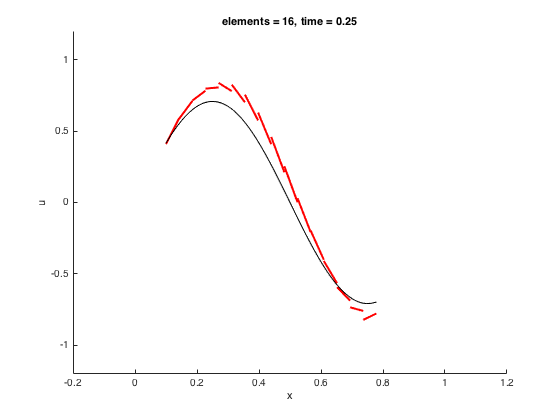
\includegraphics[width=\linewidth]{n16_t025.png}
\caption{Note that exact solution is plotted in black, the approximate in red}
\end{figure}

\begin{figure}[h]
  \centering
  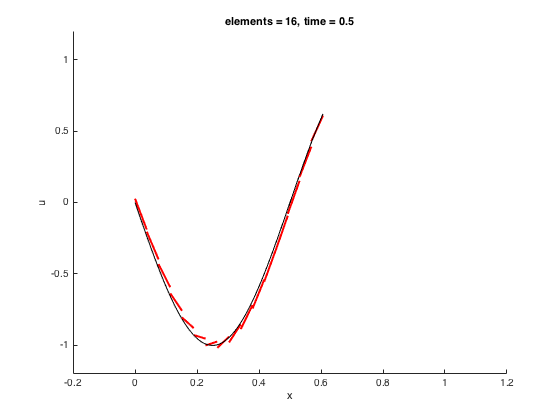
\includegraphics[width=\linewidth]{n16_t050.png}
\end{figure}

\begin{figure}[h]
  \centering
  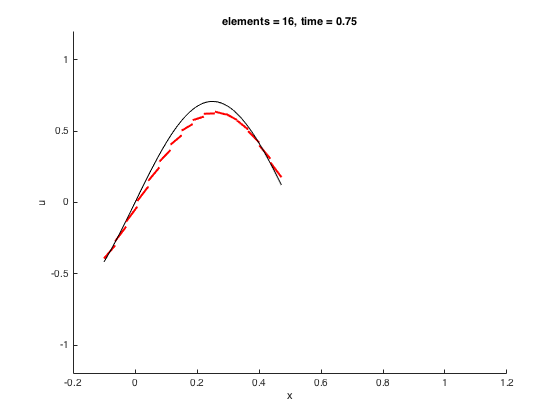
\includegraphics[width=\linewidth]{n16_t075.png}
\end{figure}

\begin{figure}[h]
  \centering
  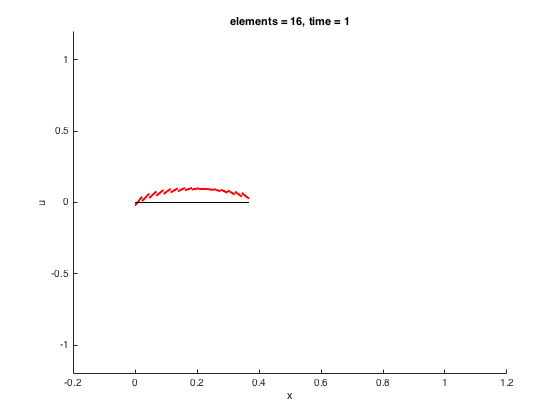
\includegraphics[width=\linewidth]{n16_t100.png}
\end{figure}

\begin{figure}[h]
  \centering
  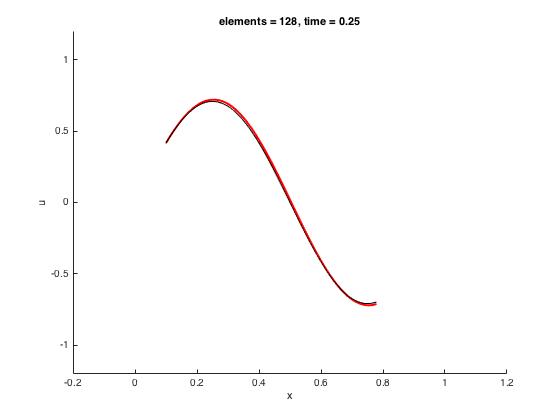
\includegraphics[width=\linewidth]{n128_t025.png}
\end{figure}

\begin{figure}[h]
  \centering
  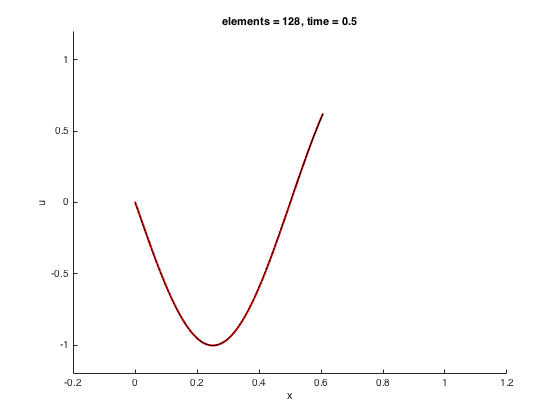
\includegraphics[width=\linewidth]{n128_t050.png}
\end{figure}

\begin{figure}[h]
  \centering
  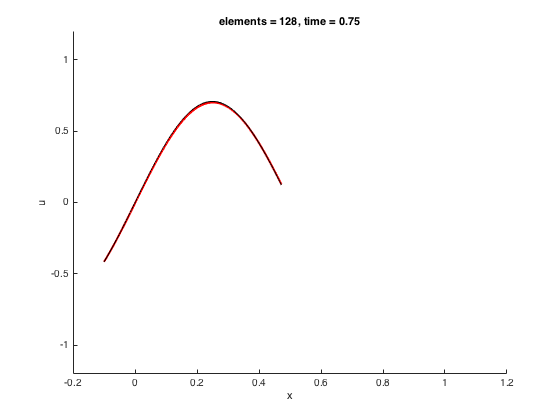
\includegraphics[width=\linewidth]{n128_t075.png}
\end{figure}

\begin{figure}[h]
  \centering
  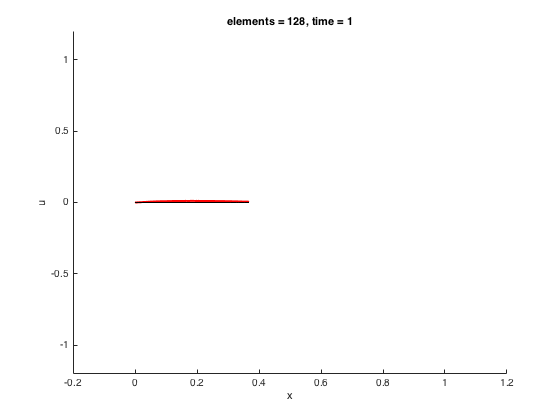
\includegraphics[width=\linewidth]{n128_t100.png}
\end{figure}


\end{document} 